\chapter{Symbolic Computer Algebra}

\section{Computations using computer algebra}

A \textit{computer algebra system} (or \textit{CAS}, for short) is software
that is able to perform algebraic procedures similar to what you would
normally do ``by hand.'' There are several popular CAS used in mathematics,
with the most common being Mathematica, Sage, and Maple. We will
be using Sage, as it is available as free open-source software, and it has been
largely developed by mathematicians, integrating many specialized packages
used by casual and professional mathematics researchers. Much of it
uses Python, so if you have any knowledge of coding in Python, you will find
Sage to be familiar; but fear not if you do not have any prior experience,
as the purpose of this lesson is to get the hang of the basics!

Sage can be installed on your computer or run from the CoCalc servers
if you create a (free) account. For now, we will use a lightweight version of Sage
that can be run on a webpage without any installation or other hassles.
 Go to \url{https://sagecell.sagemath.org/}.

You can enter basic Sage commands into the textbox on that page and
click ``Evaluate'' to get the output. We will begin by testing out some basic
arithmetic operations.

\clearpage
\begin{worksheet}{6}{Sage Cell Server}{sage.png}
Go to \url{https://sagecell.sagemath.org/}.

You can enter basic Sage commands into the textbox on the page and
click ``Evaluate'' to get the output.  To get started let's use sage like a fancy calculator.  The operands for sum, difference, multiplication, and division are \verb% +, -, *, / %.

Try the following operations:

\begin{enumerate}

\item Try the following operations:
\begin{enumerate}
	\item \verb% 1 + 2 + 3 %
	\item \verb% 42 - 23 %
	\item \verb% 1331 * 11 %
	\item \verb% 144 / 9 %
\end{enumerate}

    \item That's pretty standard stuff, you could more easily do those on your phone\dots  But, can your phone calculate 200 digits of $\pi$ in the blink of an eye?  Try this:

\begin{codeblock}
\begin{verbatim}
n(pi, digits=200)
\end{verbatim}
\end{codeblock}

    \item You may have noticed that the previous question's answers were all whole numbers, but this last one was a decimal.  We've been holding out on you a bit -- sage does {\em exact} computations.  Unless you ask it for a numerical approximation (which is what the 
    {\tt n( )} function was all about) it will give answers that are 100\% precise -- but sometimes that doesn't seem very helpful!  

    \noindent Try evaluating these:
    \begin{enumerate}
		\item \verb% pi %
		\item \verb% sqrt(2) %
		\item \verb% 7/3 %
    \end{enumerate}

    \item Sage and its brethren are Symbolic Computer Algebra Systems.  The reason it just parrots back the question to you has to do with the ``Symbolic'' part of that.  For example, the \verb+sqrt(2)+ thing above is regarded by Sage as a symbolic entity.  It is a full and precise representation of the number we write as $\sqrt{2}$.  It isn't some lame 4 or 10 or 100 digit {\em approximation} of $\sqrt{2}$. It is the real deal.  Let's see what happens when we raise \verb+sqrt(2)+ to various powers (you can use either \verb+^+ or \verb+**+ for exponentiation in sage).

	\noindent Try evaluating these:
    \begin{enumerate}
		\item \verb% sqrt(2) ^ 2 %
		\item \verb% sqrt(2) ^ 4 %
		\item \verb% sqrt(2) ^ 7 %
    \end{enumerate}

    \noindent Was the answer to that last one suprising?  Or does it make sense in retrospect?

    \item Much of the power of Computer Algebra comes from the same feature that makes regular Algebra useful -- variables.

    \noindent There are two kinds that we need to distinguish: computer variables and mathematical variables.  Computer variables are pretty easy, you can just make up whatever name you want and then start using it.  For example:

\begin{codeblock}
\begin{verbatim}
myvar = sqrt(2) ^ 7
n(myvar)
\end{verbatim}
\end{codeblock}

\noindent BTW, notice how the default version of the  {\tt n()} function only gives about 13 decimal places?  Try this too: \verb+ n(myvar, 100)+ (that's what 100 {\em bytes} of accuracy looks like -- if you want a specific number of decimal places, see the example involving $\pi$ up above.)

	\item Mathematical variables are handled a little differently.  First (other than $x$ which is there automatically) you have to declare them to the system.  The syntax looks like this: \verb+ y = var('y')+.  What's happening there is that we're telling the system that {\tt y} is a variable, but also that we want the system to print 'y' when referring to it.  I think you'll get the point if you figure out what happens when you evaluate \verb+ y = var('w') ; 6*y+.

	\item Let's try a little mathy something - with a couple of variables.  Remember how the equation of a line is usually written as $y = mx + b$?  Put the following into the sage cell:

\begin{codeblock}
\begin{verbatim}
y=var('y')
m = 2 ; b = 1
y=mx+b
\end{verbatim}
\end{codeblock}

The error message you get when evaluating this should look like:

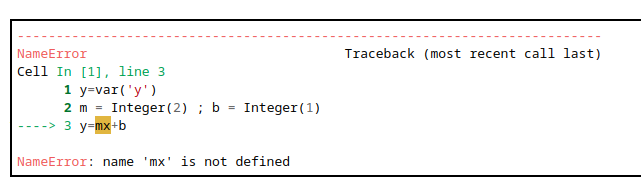
\includegraphics[scale=.5]{sage_cell-error.png}

To be fair, Sage usually puts out error messages that are on the cryptic 
side.  But not this time!  The message says ``NameError'' and it's even 
highlighted the thing that's wrong. 

%\footnote{A takeaway from this is that 
%you can't rely on implicit multiplication.  If you write \verb+7x+ the 
%system is going to think you've created a new (computer) variable whose 
%name is ``7x.''  What you really {\em meant} was \verb+7*x+ and that's 
%what you have to actually type! } 

If you fix the error, something else a little unexpected happens. Nothing!  There's no output\dots

This is just because the last line is an assignment -- it has no return value.  A very common ``idiom'' you'll see when looking at other people's sage code looks like this:

\begin{codeblock}
\begin{verbatim}
y=var('y')
m = 2 ; b = 1
y=mx+b ; y
\end{verbatim}
\end{codeblock}

\noindent The semicolon is just a way to sneak multiple commands onto a single line.  The difference here (as opposed to the code above) is that the last command isn't the assignment to the variable \verb+y+, it's just \verb+y+ by itself - and that does have a return value, namely the contents of the variable \verb+y+.



	\item Calculate $2^0$, $2^0+2^1$, $2^0+2^1+2^2$, 
		and $2^0+2^1+2^2+2^3$. Continue adding the next
		largest power of $2$ until you notice a pattern in the
		result. What is the pattern?
	
\end{enumerate}


\end{worksheet}
\clearpage



\section{Sage on CoCalc -- the interface}

For more advanced calculations that require multiple
steps, it will be beneficial to signup for CoCalc. CoCalc is a cloud-based service\footnote{``In the cloud'' really just means ``on somebody else's computer.''  There are a ton of servers out there that can be rented on flexible terms, CoCalc just purchases computing power as needed\dots} that gives its users access to many software packages.  Originally it was Sage only, but now, in addition to Sage,  one can run Python notebooks, \LaTeX{} documents, get a full Linux terminal, run a so-called ``computational whiteboard,'' even manage a course on CoCalc.  The CoCalc interface allows for sharing projects and working on thing collaboratively with one's partners -- edits become visible to the other party in real time.

Because of its genesis as a web interface to a free, open-source project, CoCalc makes free accounts available.  One can also purchase ``upgrades'' that give certain perks (most notably, access to less highly-loaded servers for your computations).  The free accounts come equipped with an ``annoyatron'' banner that urges you to get a payed account.  Many Colleges/Universities will be able to provide you with upgrade tokens so you will have the more premium experience.


This lab will lead you through the process of obtaining a CoCalc account and getting started with the Sage notebook interface.

\clearpage
\begin{worksheet}{7}{Sage on CoCalc}{sage.png}
\begin{enumerate}
	\item Go to \url{https://cocalc.com/} in a web browser.
	\item At the top right of the screen, click on the ``Sign Up''
		link.
	\item You'll need to check the box that says ``I agree to the Terms of Service.''  There is also a ``Privacy Policy'' that is included by reference into the Terms of Service.
	\item It also asks you to select the software that you plan to use.  At a minimum select ``SageMath.''  There's also an ``Everything!'' option if you feel adventurous.
	\item Next you'll be asked for your email address, your name, and to choose a password -- please make it a strong one!
	\item You should now see a page that says ``Signed in as
		XXXX XXXX'' at the top of the page.
	\item Click on the ``Projects'' link at the top left of the page.
	\item In the textbox that says, ``Project title -- you can easily change
		this at any time!'' enter a name for your new project, then
		click on the ``Create New Project'' button.
	\item On the next page, click the ``New'' link near the top
		of the page.  This is going to let you create a file inside your project.
	\item Pick a name for your file, select ``Sage worksheet,''
		then click on the ``Start project'' button at the top of the page.
	\item  Unlike in an
		embedded SageMathCell on a webpage, CoCalc will provide
		output for multiple calculations at once, and it will allow you to
		keep previous calculations on the screen so that you can
		change them or refer back to them.
	\item The interface you're looking at is called a Sage notebook. A notebook consists of an alternating sequence of input and output cells. There's a thin line between an input cell and the corresponding output cell, and the output cells have a big green border on the left side. Both sorts of cells can be shown or hidden using the little triangles in the left margin. When you first start up a fresh notebook, there is only the first input cell (with a line numbered 1 in it).  Try adding \verb%1+1% in that cell.  Watch for the pulsing green ``busy'' signal\footnote{While sage is ``thinking'' the interface provides a visual indication.  A lot of the delay is about CoCalc obtaining and setting up a fresh cloud server to run your project on, so after the first computation things should go a lot faster.} and take note of how the interface changes when you execute the cell.  (To execute, you can either hit the ``Run'' button or hold down the shift key while hitting the Enter key on your keyboard.)

	\item If you hover your mouse over the line before an input cell it will turn blue. If you then click it you'll get a new cell. It's usually a good idea to break tough computations up into manageable chunks. That's what cells are for. Just be aware that the cells in a notebook aren't independent -- if you set a variable to some value in one cell, the other cells will know about that.  Create a new cell above your \verb%1+1% cell and ask Sage to multiply a couple of random number with 10 or so digits each.  Take note of how long the
	``busy'' signal lasts this time.

	\item Let's re-emphasize a quirky thing about Sage -- assigning a value to a variable doesn't create any output. So if you want to have the computer verify that it really did what you just told it to do (i.e. print some output) you need to write the variable a second time.  This often has the form of some long computation followed by a semicolon and the name of a variable.  Try pasting the following into a new cell and hitting Shift$+$Enter.

\begin{codeblock}
\begin{verbatim}
A, P, r, n, t = var('A, P, r, n, t')
P=1000
r=.06
n=12
t=5
A = P * (1 + r/n)^(t*n) ; A
\end{verbatim}
\end{codeblock}

\item Another point that bears repeating: The instructions in a cell need to be executed in order to have any effect.  It's not enough to put your cursor in the cell and push ``Enter'' (that just adds a linebreak, making the cell longer).  You have to hold the ``Shift'' key while pressing ``Enter'' if you're trying to tell the computer to ``Do it!''  (You can also select the cell and click the ``Run'' button in the toolbar, but you'll soon find that Shift$+$Enter is a lot quicker.)

\item There are two very useful ways of getting help within sage: tab completion and help messages.  Tab completion is something you may have encountered in other computer applications. If you type the first few letters of a command and then hit the "Tab" key, the machine will either complete the typing for you, or give you a list of possible completions. Try typing "plo" in the next cell and then hitting "Tab".  You should see that Sage has a \verb+plot()+ function, but also it can do 3-dimensional plots -- and there are many other arcane-looking plots commands!

\item Ok, you just discovered that sage has a \verb+plot+ command -- but how do you use it? For that, it's often a good idea to look at the help message for the command. To get help, just type a question mark after the name of the command (then "Shift+Enter").

\noindent I usually just scroll down through the help message until I find some examples\dots

\item Speaking of examples, the tool bar above the cells is full of them!  Create a fresh cell, then find the ``Plots'' drop-down and select ``Function''  Hit Shift$+$Enter and you should see something like:

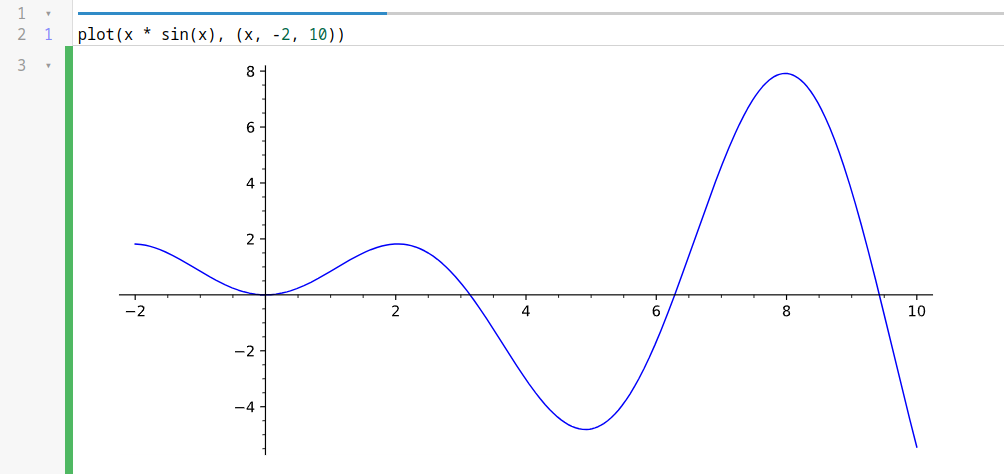
\includegraphics[scale=.4]{first_plot_screenshot.png}

\item Even more help is accessible from the top menu entry that's labelled, uhmmm, ``Help.''  There you can access the sage documentation, submit a support ticket if you think you've found a bug, or even have a chat with ChatGPT.  Try it!

\item When executing a cell produces an error message you can even ask for ``Artificial Intelligence help'' in correcting the problem.  It's possible to hold a back-and-forth conversation with ChatGPT that feels almost like talking to a human!

\item Some of you have probably already studied Calculus.  For others it will be coming up soon! The two main operations in Calculus (which are in a certain sense inverses of one another) are known as integration and differentiation.  Try using tab-completion and the help facility to find out how to do these operations in Sage.  It's pretty likely that you'll do something incorrect and get an error message.  If that happens try the ``Ask ChatGPT'' option.  Turn it into a conversation where you go back and forth with the AI a few times!

\end{enumerate}

\end{worksheet}
\clearpage

\section{Sage on CoCalc II -- Algebra}

The last lab mostly concentrated on getting you used to the interface. Of course, learning that interface would be pointless if Sage wasn't capable of doing something useful for us!

And it {\em definitely} can!

The next lab has us exploring Sage's abilities in Algebra.  Recall the operations with polynomials that you learned to do by hand in Algebra class:

\begin{itemize}
	\item Multiplying 2 polynomials (do you recall the FOIL mnemonic?)
	\item Factoring a polynomial (sort of the opposite of the previous thing)
	\item Evaluating a polynomial at a particular value of its variable.
	\item Solving -- what $x$ values give a particular output?
\end{itemize}

Not to say that that was wasted effort (if nothing else, your brains got stronger from the exercise!)
but, yeah, Sage can do all of that and more\dots

Before we jump into the actual lab, a quick word about ``equals.''

There's really just one version of the ``equality'' idea in Mathematics.  In Computing, there are two:
\begin{enumerate}
	\item One place an equals sign shows up is when we're assigning a value to a variable.
	\item The other place an equals sign shows up is when we're checking whether two variables actually contain the same content.
\end{enumerate}

In Sage (and Python) the ``assignment'' version uses a single ``$=$'' -- the ``equality testing'' sense use a double ``$==$.''  

If you were to execute 

\begin{codeblock}
\begin{verbatim}
x=1
x==0
\end{verbatim}
\end{codeblock}

\noindent in a Sage cell, the first line (being an assignment) will produce no output, and the second line will produce output informing us that {\em no} - one and zero are not the same.


\begin{worksheet}{8}{Sage on CoCalc II -- Algebra}{sage.png}

Most of the computations we did in the previous section can be
done on a regular calculator, but where a CAS like Sage really
shines is when working with algebraic expressions including
variables. When working with Sage, we will need to declare
symbolic variables before we use them.

\begin{verbatim}
x = var('x')
\end{verbatim}

This tells Sage that we will be using the symbol/letter ``x'' as an
unbound variable in an expression. We wish to treat it as symbol
that can represent any possible value and not as a specific
value that is fixed.  In other words, $x$ is a mathematical variable, not a computer variable.

\begin{verbatim}
x = var('x')
3*x+7*x+5
\end{verbatim}

This represents the expression $3x+7x+5$. Note that the implied
multiplication between $3$ and $x$ needs to be specified when
typing into Sage.

Inputting

\begin{verbatim}
var('x')
3x
\end{verbatim}

\noindent will just cause a NameError.

Sage can be helpful when working with algebraic expressions, as
it can do things like expand, factor, or simplify expressions.

If we want to factor an expression like $x^2+4x+3$, we can use
the  {\tt factor} command.

\begin{verbatim}
x=var('x')
factor(x^2+4*x+3)
\end{verbatim}

We can also expand out an expression using the {\tt expand} command.

\begin{verbatim}
x=var('x')
expand( (x+1)*(x+3) )
\end{verbatim}

It is also often useful to define a function, such as $f(x)$, much like
we do in a regular math class.

\begin{verbatim}
x=var('x')
f(x)=x^2+4*x+3
\end{verbatim}

We can then evaluate $f(x)$ at different values of $x$ using the standard
notation. For example, to evaluate at $x=1$, we can then enter

\begin{verbatim}
f(1)
\end{verbatim}

which will give us the output of

\begin{verbatim}
8
\end{verbatim}

which is the same as the value of $(1)^2+4(1)+3$, i.e. the value of
substituting $x=1$ into $f(x)=x^2+4x+3$.

We can also easily apply the {\tt expand} and {\tt factor}
commands to a function we have already defined.

\begin{verbatim}
f.factor()
\end{verbatim}

will give the output

\begin{verbatim}
x |--> (x+3)*(x+1)
\end{verbatim}

which is the same factorization as when we typed

\begin{verbatim}
factor(x^2+4*x+3)
\end{verbatim}

Similarly,

\begin{verbatim}
f.expand()
\end{verbatim}

can be used to {\tt expand} the function $f(x)$. In addition,
a function has the {\tt full\_simplify} option.

\begin{verbatim}
var('x')
f(x)=(x^2+4*x+3)/x+(x+3)*(x-1)/(x+1)
f.full_simplify()
\end{verbatim}

Will simplify the very complicated expression of
\begin{equation*}
	\frac{x^2+4x+3}{x} + \frac{(x+3)(x-1)}{x+1}
\end{equation*}
into a single rational function.

Finally, sometimes Sage will give us an exact expression for
something for which we would like a decimal approximation.
For example, 

\begin{verbatim}
var('x')
f(x)=(x^2+4*x+3)/x+(x+3)*(x-1)/(x+1)
f(2)
\end{verbatim}

gives the output

\begin{verbatim}
55/6
\end{verbatim}

Because Sage is mathematical software, and mathematicians usually
want exact answers, that is what it will return, when possible. In order
to force it to give a decimal expression, we can use the
{\tt n()} command.

\begin{verbatim}
n(55/6)
\end{verbatim}

gives the decimal approximation of

\begin{verbatim}
9.16666666666667
\end{verbatim}


\end{worksheet}
\clearpage

\begin{worksheet}{9}{Finding Solutions in Sage}{sage.png}
{\bf \large Solving equations}

(Note: follow along with these initial computations then try the problems.)

We will investigate functions of the form $f(x)=ax^2+bx+c$. To begin
with, we will consider when $a=1$, $b=0$, and $c=0$, i.e. $f(x)=x^2$.


Start by defining $f(x)=x^2$ in Sage.

\begin{verbatim}
f(x)=x^2
\end{verbatim}

To solve the equation $f(x)=1$ (i.e. $x^2=1$) in Sage, we can use the
\textbf{solve} command:

\begin{verbatim}
solve(f(x)==1, x)
\end{verbatim}

This will solve the equation $f(x)=1$, solving for the variable $x$.
Note that when solving, we need to put two equals signs to denote
equality. This is because Sage will interpret a single equals sign
as an assignment (i.e. we would be defining $f(x)$ to be the function
that is always equal to $1$).

The output we obtain is

\begin{verbatim}
[x == -1, x == 1]
\end{verbatim}

These are the two solutions that we expect of $x=-1$ and $x=1$.

{\bf Exercises}

\begin{enumerate}
	\item Try to solve the equation $f(x)=4$ using Sage.
	\item Solve the equation $f(x)=3$ using Sage.
	\item Solve the equation $f(x)=0$ using Sage.
	\item Do you expect for there to be any solutions for $f(x)=-9$?
		Try it in Sage and see what happens.
	\item For what values of $h$ does $f(x)=h$ have two real solutions?
		Only 1 solution? Two imaginary solutions?
	\item Define a new function $g(x) = x^2 + 10x + 21$.  Let's try two things:
	\begin{enumerate}
		\item Use the \verb+factor()+ member function to see how $g(x)$ factors.
		\item Use the \verb+solve()+ command to see when $g(x)$ is equal to zero.
	\end{enumerate}
	Can you explain the minus signs?

	\item Do the things \verb+factor()+ and \verb+solve()+ in the previous problem for 
	\begin{enumerate}
		\item $g(x) = x^2 + 10x + 22$
		\item $g(x) = x^2 + 10x + 23$
		\item $g(x) = x^2 + 10x + 24$
		\item $g(x) = x^2 + 10x + 25$
		\item $g(x) = x^2 + 10x + 26$
	\end{enumerate}

    Sometimes Sage factors the polynomial into linear factors. \newline
    Sometimes Sage is refusing to factor because the zeros are not nice numbers.\newline
    Once, Sage refuses to factor because things have gotten truly weird.

    Identify which is which?  What do you suppose \verb+I - 5+ means?

\end{enumerate}

{\bf \large Graphing functions}

(Again, follow along with the first few computations, then try the problems.)

Another useful way to analyze things is by visualizing functions using plots of their graphs. Let's begin by plotting the function $f(x)=x^2$:

\begin{verbatim}
f(x)=x^2
plot(f(x))
\end{verbatim}

The first line defines the function $f(x)=x^2$, then the second line will plot
the function. Note that since we did not specify the range for the axes, the
plot will automatically pick a range. If we want to see more of the graph, we
can try adjusting the \textbf{xmin}, \textbf{xmax}, \textbf{ymin}, and \textbf{ymax}
values, which correspond to the minimum and maximum values of the
$x$- and $y$- axes that we desire. For example, changing the plot
command to

\begin{verbatim}
plot(f(x),xmin=-3,xmax=3,ymin=-2,ymax=9)
\end{verbatim}

will gives us an $x$-axis that ranges from $-3$ to $3$ and a $y$-axis that
ranges from $-2$ to $9$.

We can also plot multiple functions on the same plot, in case we
want to compare them together. Let's try overlaying the graph of
the function $g(x)=1$ onto the same set of axes:

\begin{verbatim}
f(x)=x^2
g(x)=1
plot([f(x), g(x)],xmin=-3,xmax=3,ymin=-2,ymax=9)
\end{verbatim}

We have defined two functions now, $f(x)=x^2$ and $g(x)=1$. To
plot both, we put them both into a list that is enclosed in square
brackets, with the two functions separated by a comma. This produces
graphs of both $f(x)$ and $g(x)$, in two different colors.

How many times do the graphs of $f(x)$ and $g(x)$ intersect?

{\bf Exercises}

\begin{enumerate}
	\item Graph the functions $f(x)=x^2$ and $g(x)=4$ together
		on the same set of axes. How many times do the
		graphs of $f(x)$ and $g(x)$ intersect?
	\item Repeat with $f(x)=x^2$ and $g(x)=3$. How many times do the
		graphs of $f(x)$ and $g(x)$ intersect?
	\item Repeat with $f(x)=x^2$ and $g(x)=0$. How many times do the
		graphs of $f(x)$ and $g(x)$ intersect?
	\item Repeat with $f(x)=x^2$ and $g(x)=-3$. How many times do the
		graphs of $f(x)$ and $g(x)$ intersect?
	\item What is the relationship between the number of times
		that the graphs of $f(x)=x^2$ and $g(x)=k$ intersect and the
		number of solutions to $x^2=k$?
	\item Are there any intersections of the graphs $f(x) = x^2 + 1$ and $g(x) = x+2$ ? \newline
	Use a sage \verb+plot()+ command to visualize the situation, then use the \verb+solve()+ command to find the points of intersection. 
	\item Notice that in the last problem the \verb+solve()+ command only gives us the $x$ coordinates of the points of intersection.  How can we find the $y$ coordinates?
    \item Recall that the quadratic formula is 

    \[  \frac{-b \pm \sqrt{b^2 - 4ac}}{2a}. \]

    What are the $a$, $b$ and $c$ in this case?  Careful! You need to rearrange so that you have a quadratic polynomial set equal to zero.

    Does the answer from using Sage's \verb+solve()+ command agree with what the quadratic formula tells us?
\end{enumerate}

{\bf \large Numerical Approximations to Solutions of Equations}

(There are no problems in this section, so just read along and do the computations as you encounter them.)

Some equations are difficult to solve exactly even with the
assistant of a computer and computer software, and Sage is no
exception to this. 

Use the \textbf{solve} function to have Sage solve the
equation $x^5-3x^4+x^3+2=0$. 

The output that we get is
\begin{verbatim}
[0 == x^5 - 3*x^4 + x^3 + 2]
\end{verbatim}

which is another way of Sage telling us that it could not find a solution.
However, plotting the function $x^5-3x^4+x^3+2$ tells us another story.
Plot the graph of $x^5-3x^4+x^3+2$ in Sage to see whether it has
any roots. How many are there, and what are the approximate values
from the graph? You may want to play around with the range of the
$x$-axis (using xmin and xmax) to get a clearer picture.

(3 roots, roughly -0.8, 1.2, and 2.5)

We see that there are 3 roots, at roughly $x=-0.8$, $1.2$, and $2.5$.
Although Sage cannot get the exact values for them by solving
the equation $x^5-3x^4+x^3+2=0$, it can get approximate decimal
values for the roots by using the \textbf{find\_root} function. In
short, a computer algebra system such as Sage uses a sophisticated
version of "find where the graph crosses the $x$-axis, and zoom in
repeatedly around that point to get a more precise estimate of the
$x$-coordinate of where the graph crosses the $x$-axis.'' To find
a root $x$ where $-2<x<0$, we would use the command

\begin{verbatim}
find_root(x^5-3*x^4+x^3+2==0, -2, 0)
\end{verbatim}

The output of this is the root

\begin{verbatim}
-0.7931397744702121
\end{verbatim}

If we want to find a different root, we can change the interval on
which we instruct Sage to look for a root. For example, if we want
to find the root near $1.2$, we could try something like

\begin{verbatim}
find_root(x^5-3*x^4+x^3+2==0, 1, 2)
\end{verbatim}

which gives us the value

\begin{verbatim}
1.199258801379252
\end{verbatim}

Try to find the approximate value of the root of $x^5-3x^4+x^3+2$
near $x=2.5$.

(value is 2.563623765649018)

Note that we said that these values are approximate. Let's verify
what we mean by that. Recall that a root of a function $f(x)$ is
a value of $x$ that makes $f(x)$ equal to exactly $0$, i.e.
$f(x)=0$. Use Sage to define the function $f(x)=x^5-3x^4+x^3+2$,
then plug in the values of the approximate roots from above,
e.g. find $f(-0.7931397744702121)$. If $-0.7931397744702121$
is truly a solution to $x^5-3x^4+x^3+2=0$, then
$f(-0.7931397744702121)$ should equal exactly 0.

However, the value that we get from Sage is

\begin{verbatim}
1.35419453428653e-13
\end{verbatim}

The $e$ here is used for \underline{e}ngineering notation,
where 1.35419453428653e-13 means
\begin{equation*}
1.35419453428653\times 10^{-13}
\end{equation*}

In other words, the part before the ``e'' is a decimal number,
but then the part after the ``e'' is the exponent that we should
raise $10$ to then multiply the decimal. Another way to think of
this is that the ``e-13'' means we should start with the
1.35419453428653 then move the decimal to the left 13 times,
making our number smaller. In contrast, if we had seen

\begin{verbatim}1.35419453428653e5\end{verbatim}

that would mean move the decimal to the right 5 places, resulting
in the number $135419.453428653$.

The number $1.35419453428653\times 10^{-13}$ is a really
small number, but it's not exactly equal to 0. This 
demonstrates that the decimal ``solution'' we obtained using
\textbf{find\_root} is only approximate and not an exact solution.

Another thing to be cautious about when using \textbf{find\_root}
is that it will quit as soon as it finds one approximate root. In other
words, even if there is another root in the interval that you specify,
\textbf{find\_root} will only tell you the value of one of them. If we
try

\begin{verbatim}
find_root(x^5-3*x^4+x^3+2==0, 1, 3)
\end{verbatim}

in hopes of finding both roots that are between 1 and 3, it will not
give us both. Try this out and see what you get!

(only the solution 2.563623765649033 is found)

\end{worksheet}
\clearpage

Lab 10 is entirely on CoCalc.  A Sage worksheet file is available on the book website. 

\section{Projects}

The projects for this section will be individual.  Pick one of the following and be prepared to give a presentation on what you did.

\subsection{Create an amazing graphic to use as the ``end of lab'' marker.}

Do that.

P.S. Just copying one of the examples and changing the colors will not be sufficient!

\subsection{Pascal's triangle}

In Lab 9, you may have noticed that the pattern of the coefficients of $(x+y)^n$ yielded a familiar thing known as Pascal's triangle.  Do some research and write a short paper (3-4 pages in Overleaf) about Pascal's triangle explaining how the triangle works to the rest of us.  Here's a few questions you may want to look for answers for:

\begin{enumerate}
	\item Who was Pascal and why did he create this triangle?
	\item What is the recursive rule that gives a row of the triangle in terms of the one above it?
	\item What is the sum of the entries in a row of Pascal's triangle?  Why?
	\item Why are the entries sometimes called ``choice counters''?
	\item The hockeystick theorem?
	\item There's a cool pattern that arises if we color the entries in the triangle based on the remainder we get when dividing by some agreed upon number. ( I know that's not really a question.)
\end{enumerate}

\subsection{The quadratic formula}

Take your pick.  Write a 3-4 page paper in Overleaf or create a Webpage on Google Sites (using jsmath for any mathematical notation) explaining what the quadratic formula is. Also, what it's for. And, how did they derive it?
A bit of historical research would be reasonable -- when did humans first learn this magic?  Is there any debate about that?  How is the quadratic formula related to the process known as ``completing the square.''?  Use sage to compute some examples and also to generate some graphics to include in your paper/website.


\subsection{Iterating functions and chaos}

Consider what happens when one applies the function $g(x)=-rx^2+rx$
to a number repeatedly.

We will start when $r=0.5$, so that $g(x)=-0.5x^2+0.5x$. Given that choice for $r$ we will use the initial value $x=2$. What is the value of $g(2)$? $g(g(2))$? $g(g(g(2))$?
If we continue to apply $g$ more and more times to the result, what eventually
happens to the output? Use Sage to make your calculations. You may want to
apply \textbf{n()} to your output to get a decimal value to more easily
see the pattern.

Now change $x$ to any number of your choice and repeat the experiment of
applying $g$ repeatedly. What is the eventual outcome?

(all initial values converge to $0$)

Now consider when $r=1.2$, i.e. $g(x)=-1.2x^2+1.2x$.
Start with an initial value of your choice and repeat
the experiment of applying $g$ repeatedly. What is the eventual outcome?

(all initial values converge to $\frac{r-1}{r}=0.1\bar{6}$)

To track the results of iteratively applying the function $g(x)$ to an initial
value of $x=a$, we can create a list of values.

\begin{verbatim}
var('x')
g(x)=-0.5*x^2+0.5*x

a=0.5

points = [a, g(a), g(g(a)), g(g(g(a))), g(g(g(g(a)))), g(g(g(g(g(a)))))]
\end{verbatim}

We can then plot this using the \textbf{list\_plots} function.

\begin{verbatim}
list_plot(points)
\end{verbatim}

If we want to change the value of $a$, we can easily do so, then re-run
the commands that come after it. In addition, if we want to see what
happens when we apply $g(x)$ more times, we can also add those
extra iterates to the list to get a better visualization of what happens
to the output as we apply $g(x)$ more and more times.

Play around with different values of $r$ between $2$ and $4$ and any
choice of the initial value $x$. What patterns do you notice?

Now let's fix a value of $r=3.5$, so we are looking at the function
$g(x)=-3.5x^2+3.5x$. Pick two different values of $x$ that are close to each other 
(within $0.1$ of each other) and plot repeated iterates of $g(x)$ on separate
graphs. What do you notice?
What happens as the two values of $x$ get closer and closer together?

We note that the values seem to be clustered around 4 different values,
and that the iterates seem to cycle through the values systematically. This is called
a \textit{periodic orbit}, and in particular, this is a periodic orbit of length 4 because
the values (approximately) repeat every 4 times that we apply $g$. To find
the periodic points, we can solve for when $x=g(g(g(g(x))))$. Find the points
in this periodic orbit by solving $x=g(g(g(g(x))))$ using Sage.

Write up your findings in a 3-4 page \LaTeX paper on overleaf.